%\documentstyle[11pt,fullpage]{article}
%\setlength{\parindent}{0 in}
%\setlength{\parskip}{.1in}
%\setlength{\topmargin}{-0.5in}
%\setlength{\textheight}{8.5in}
%\begin{document}
\chapter{Satellite Networking in \ns}
\label{chap:satellite}

This chapter describes extensions that enable the simulation of satellite
networks in \ns.  In particular, these extensions enable \ns~to model
the following:  i) traditional geostationary ``bent-pipe'' satellites with 
multiple users per uplink/downlink and asymmetric links, ii) geostationary 
satellites with processing payloads (either regenerative payloads or full 
packet switching), and iii) polar orbiting LEO constellations such as 
Iridium and Teledesic.  These satellite models are principally aimed at 
using \ns~to study networking aspects of satellite systems; in particular, 
MAC, link layer, routing, and transport protocols.  

%\paragraph{Notice (caveat emptor)} 

%This code (including perhaps the APIs at OTcl level) is likely to change 
%over the next few months (as of this writing in June 1999) as the \ns~
%developers work on integrating the structure of satellite nodes, 
%wireless nodes, hierarchical nodes, etc.  In particular, we plan on
%modifying the code to support mixed-node topologies (e.g., simulations
%consisting of traditional \ns~nodes and satellite nodes) and running existing 
%unicast and multicast OTcl-based routing protocols.  \nam~~is 
%not currently supported with these extensions.

%%%%%%%%%%%%%%%%%%%%%%%%%%%%%%%%%%%%%%%%%%%%%%%%%%%%%%%%%%%%%%%%%%%%%%%%%%
%%%%%%%%%%%%%%%%%%%%%%%%%%%%%%%%%%%%%%%%%%%%%%%%%%%%%%%%%%%%%%%%%%%%%%%%%%

\section{Overview of satellite models}
\label{sec:satellite/overview}

Exact simulation of satellite networks requires a
detailed modelling of radio frequency characteristics (interference, fading),
protocol interactions (e.g., interactions of residual burst errors on the 
link with error checking codes), and second-order orbital effects (precession,
gravitational anomalies, etc.).  However, in order to study fundamental
characteristics of satellite networks from a {\em networking} perspective,
certain features may be abstracted out.  For example, the performance of
TCP over satellite links is impacted little by using an approximate rather than 
detailed channel model-- performance can be characterized to first order
by the overall packet loss probability.  This is the approach taken in this
simulation model-- to create a framework for studying transport, 
routing, and MAC protocols in a satellite environment consisting of
geostationary satellites or constellations of polar-orbiting 
low-earth-orbit (LEO) satellites.  Of course, users may extend these models
to provide more detail at a given layer.   

%%%%%%%%%%%%%%%%%%%%%%%%%%%%%%%%%%%%%%%%%%%%%%%%%%%%%%%%%%%%%%%%%%%%%%%%%%

\subsection{Geostationary satellites}
\label{sec:satellite/overview/geo}

Geostationary satellites orbit the Earth at an altitude of 22,300 miles 
above the equator.  The position of the satellites is specified in terms
of the longitude of the nadir point (subsatellite point on the Earth's
surface).  In practice, geostationary satellites can drift from their
designated location due to gravitational perturbations-- these effects
are not modelled in \ns.   

Two kinds of geostationary satellites can be modelled.  Traditional
``bent-pipe'' geostationary satellites are merely repeaters in orbit--
all packets received by such satellites on an uplink channel are piped
through at RF frequencies to a corresponding downlink, and the satellite node
is not visible to routing protocols.   Newer satellites will
increasingly use baseband processing, both to regenerate the digital signal and
to perform fast packet switching on-board
the spacecraft.  In the simulations, these satellites can be modelled more like 
traditional \ns~nodes with classifiers and routing agents.  
  
Previously, users could simulate geostationary satellite links by simply
simulating a long delay link using traditional \ns~links and nodes.  The
key enhancement of these satellite extensions with respect to geostationary
satellites is the capability to simulate MAC protocols.  Users can now
define many terminals at different locations on the Earth's surface and
connect them to the same satellite uplink and downlink channels, and the
propagation delays in the system (which are slightly different for each
user) are accurately modelled.  In addition, the uplink and downlink channels
can be defined differently (perhaps with different bandwidths or error models).

%%%%%%%%%%%%%%%%%%%%%%%%%%%%%%%%%%%%%%%%%%%%%%%%%%%%%%%%%%%%%%%%%%%%%%%%%%

\subsection{Low-earth-orbiting satellites}
\label{sec:satellite/overview/leo}

\begin{figure}
    \centerline{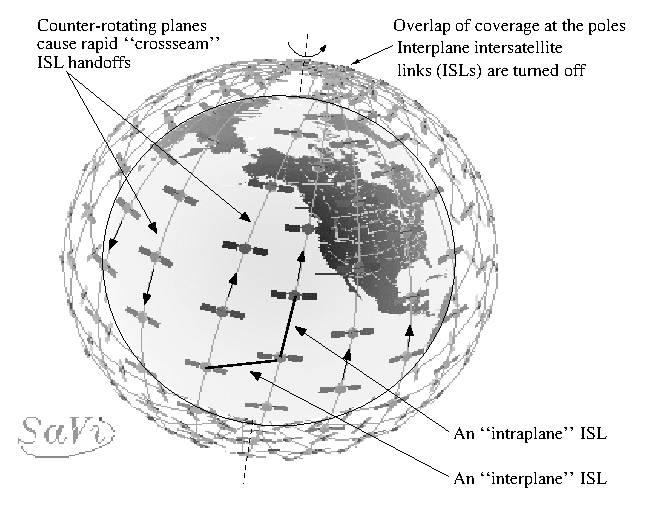
\includegraphics{sat-constellation}}
    \caption{Example of a polar-orbiting LEO constellation.  This figure
was generated using the SaVi software package from the geometry center at the
University of Minnesota.}
    \label{fig:constellation}
\end{figure}

Polar orbiting satellite systems, such as Iridium and the proposed Teledesic 
system, can
be modelled in \ns.   In particular, the simulator supports the specification
of satellites that orbit in purely circular planes, for which the neighboring 
planes are co-rotating.
There are other non-geostationary constellation configurations  
possible (e.g., Walker constellations)-- the interested user may develop new
constellation classes to simulate these other constellation types.  In
particular, this would mainly require defining new intersatellite link 
handoff procedures.

The following are the parameters of satellite constellations that can currently
be simulated:
\begin{itemize}
        \item {\bf Basic constellation definition} Includes satellite altitude,
number of satellites, number of planes, number of satellites per plane.
        \item {\bf Orbits} Orbit inclination can range continuously
from 0 to 180 degrees (inclination greater than 90 degrees corresponds to
retrograde orbits).  Orbit eccentricity is not modeled.  Nodal precession is 
not modeled.  Intersatellite spacing within a given plane is fixed.  Relative
phasing between planes is fixed (although some systems may not control phasing
between planes).
        \item {\bf Intersatellite (ISL) links} For polar orbiting 
constellations,
intraplane, interplane, and crossseam ISLs can be defined.  Intraplane ISLs
exist between satellites in the same plane and are never deactivated or 
handed off.  Interplane ISLs exist between satellites of neighboring 
co-rotating planes.  These links are deactivated near the poles (above
the ``ISL latitude threshold'' in the table) because the antenna pointing 
mechanism cannot track these links in the polar regions.  Like intraplane ISLs,
interplane ISLs are never handed off.  Crossseam ISLs may exist in a 
constellation between satellites in counter-rotating planes (where the 
planes form a so-called ``seam'' in the topology).   GEO ISLs can also be
defined for constellations of geostationary satellites.
        \item {\bf Ground to satellite (GSL) links}  Multiple terminals
can be connected to a single GSL satellite channel.  GSL links for GEO 
satellites are static, while GSL links for LEO channels are periodically 
handed off as described below.  
        \item {\bf Elevation mask} The elevation angle above which a GSL 
link can be operational.  Currently, if the (LEO) satellite serving a terminal
drops below the elevation mask, the terminal searches for a new satellite
above the elevation mask.  Satellite terminals check for handoff opportunities
according to a timeout interval specified by the user.  Each terminal
initiates handoffs asynchronously; it would be possible also to define
a system in which each handoff occurs synchronously in the system.
\end{itemize}

The following table lists parameters used for example simulation scripts
of the Iridium\footnote{Aside
from the link bandwidths (Iridium is a narrowband system only), these
parameters are very close to what a broadband version of the Iridium system
might look like.}  and Teledesic\footnote{These Teledesic constellation 
parameters are subject to change; 
thanks to Marie-Jose Montpetit of Teledesic for providing
tentative parameters as of January 1999.  The link bandwidths are not
necessarily accurate.} systems.

\begin{table}[h]
\begin{center}
{\tt
\begin{tabular}{|c||c|c|}\hline
& {\bf Iridium} & {\bf Teledesic}\\\hline\hline
{\bf Altitude} & \rm 780 km& \rm 1375 km\\\hline
{\bf Planes} & \rm 6& \rm 12\\\hline
{\bf Satellites per plane} & \rm 11 & \rm 24\\\hline
{\bf Inclination (deg)} & \rm 86.4 & \rm 84.7\\\hline
{\bf Interplane separation (deg)} & \rm 31.6 & \rm 15\\\hline
{\bf Seam separation (deg)} & \rm 22 & \rm 15\\\hline
{\bf Elevation mask (deg)} & \rm 8.2 & \rm 40\\\hline
{\bf Intraplane phasing} & \rm yes & \rm yes\\\hline
{\bf Interplane phasing} & \rm yes & \rm no\\\hline
{\bf ISLs per satellite} & \rm 4  & \rm 8\\\hline
{\bf ISL bandwidth} & \rm 25 Mb/s  & \rm 155 Mb/s\\\hline
{\bf Up/downlink bandwidth} & \rm 1.5 Mb/s  & \rm 1.5 Mb/s\\\hline
{\bf Cross-seam ISLs} & \rm no & \rm yes\\\hline
{\bf ISL latitude threshold (deg)} & \rm 60 & \rm 60\\\hline
\end{tabular}
}
\end{center}
\caption{Simulation parameters used for modeling a broadband version of
the Iridium system and the proposed 288-satellite Teledesic system.
Both systems are examples of polar orbiting constellations.
}
\end{table}
\clearpage
%%%%%%%%%%%%%%%%%%%%%%%%%%%%%%%%%%%%%%%%%%%%%%%%%%%%%%%%%%%%%%%%%%%%%%%%%%
%%%%%%%%%%%%%%%%%%%%%%%%%%%%%%%%%%%%%%%%%%%%%%%%%%%%%%%%%%%%%%%%%%%%%%%%%%

\section{Using the satellite extensions}
\label{sec:satellite/usage}

\begin{figure}
    \centerline{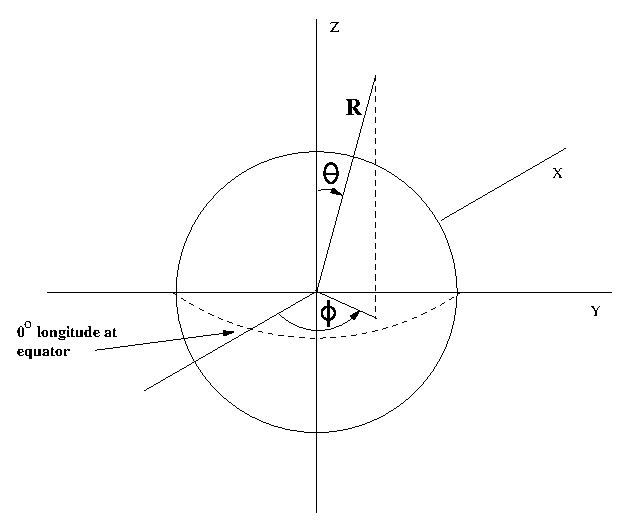
\includegraphics{sat-spherical}}
    \caption{Spherical coordinate system used by satellite nodes}
    \label{fig:spherical}
\end{figure}

%%%%%%%%%%%%%%%%%%%%%%%%%%%%%%%%%%%%%%%%%%%%%%%%%%%%%%%%%%%%%%%%%%%%%%%%%%

\subsection{Nodes and node positions}
\label{sec:satellite/usage/nodes}

There are two basic kinds of satellite nodes:  {\em geostationary}  
and {\em non-geostationary} satellite nodes.  In addition, {\em terminal} nodes
can be placed on the Earth's surface.  As is explained later in 
Section \ref{sec:satellite/implementation},
each of these three different types of nodes is actually implemented with 
the same \code{class SatNode} object, but with different position,
handoff manager,  and link objects attached.  
The position object keeps track of the satellite node's location 
in the coordinate system as a function of the elapsed simulation time.
This position information is used to determine link propagation delays and
appropriate times for link handoffs.  Section~\ref{sec:node:nodeconfig} 
introduced the 
"node-config" utility used to prime the node generator for different
types of satellite nodes. 

Figure \ref{fig:spherical} illustrates the spherical coordinate system,
and the corresponding Cartesian coordinate system.
The coordinate system is centered at the 
Earth's center, and the $z$ axis coincides with the Earth's axis of rotation.  
$(R,\theta,\phi) = (6378 km, 90^o, 0^o)$ corresponds to $0^o$ longitude 
(prime meridian) on the equator.

Specifically, there is one class of satellite node \code{Class Node/SatNode},
to which one of three types of \code{Position} objects may be attached.  
Each \code{SatNode} and \code{Position} object is a split OTcl/C++ object,
but most of the code resides in C++.  The following types of position objects 
exist: 
\begin{itemize}
\item \code{Position/Sat/Term} A terminal is specified by its latitude and
longitude.  Latitude ranges from $[-90, 90]$ and longitude ranges from
$[-180, 180]$, with negative values corresponding to south and west, 
respectively.  As simulation time evolves, the terminals move along
with the Earth's surface.  The  node generator can be used 
to create a terminal with an attached position object as follows:
\begin{program}
$ns node-config -satNodeType terminal \bs
		(other node config commands go here...)
set n1 [$ns node]
$n1 set-position $lat $lon; # in decimal degrees
\end{program}
\item \code{Position/Sat/Geo} A geostationary satellite is specified by its 
longitude above the equator.  As simulation time evolves, the geostationary
satellite moves through the coordinate system with the same orbital period
as that of the Earth's rotation.  The longitude ranges from $[-180,180]$
degrees.  As we describe further below, two flavors of geostationary nodes
exist:  ``geo'' (for processing satellites) and ``geo-repeater'' (for bent-pipe
satellites).  The node generator can be
used to create a geostationary satellite with an attached position object as 
follows:
\begin{program}
$ns node-config -satNodeType geo (or ``geo-repeater'') \bs
		(other node config commands go here...)
set n1 [$ns node]
$n1 set-position $lon; # in decimal degrees
\end{program}
\item \code{Position/Sat/Polar} A polar orbiting satellite has a purely
circular orbit along a fixed plane in the coordinate system; the Earth
rotates underneath this orbital plane, so there is both an east-west and
a north-south component to the track of a polar satellite's footprint on
the Earth's surface.  Strictly speaking, the polar position object can
be used to model the movement of any circular orbit in a fixed plane;  
we use the term ``polar'' here because we later use such satellites to model 
polar-orbiting constellations.

Satellite orbits are usually specified by six parameters:  {\em altitude},
{\em semi-major axis}, {\em eccentricity}, 
{\em right ascension of ascending node}, {\em inclination}, and
{\em time of perigee passage}.  The polar orbiting satellites in \ns~have
purely circular orbits, so we simplify the specification of the orbits to
include only three parameters: {\em altitude}, {\em inclination}, and
{\em longitude}, with a fourth parameter {\em alpha} specifying initial 
position of the satellite in the orbit, as described below.
{\bf Altitude} is specified in kilometers above the Earth's surface, and 
{\bf inclination} can range from $[0,180]$ degrees, with $90$ corresponding
to pure polar orbits and angles greater than $90$ degrees corresponding
to ``retrograde'' orbits.  The {\em ascending node} refers to the point
where the footprint of the satellite orbital track crosses the equator 
moving from south to north.  In this simulation model, the parameter 
{\bf longitude of ascending node} specifies the earth-centric longitude at 
which the satellite's nadir point crosses the equator moving south
to north.\footnote{Traditionally, the ``right ascension'' of the ascending
node is specified for satellite orbits-- the right ascension corresponds to the 
{\em celestial} longitude.  In our case, we do not care about the
orientation in a celestial coordinate system, so we specify the earth-centric
longitude instead.} {\em Longitude of ascending node} can range from 
$[-180,180]$ degrees.  The fourth parameter,
{\bf alpha}, specifies the initial position of the satellite along this
orbit, starting from the ascending node.  
For example, an {\em alpha} of $180$ degrees indicates that the
satellite is initially above the equator moving from north to south.
{\em Alpha} can range from $[0,360]$ degrees.
Finally, a fifth parameter, {\bf plane}, is specified when creating
polar satellite nodes-- all satellites in the same plane are given the
same plane index.
The node generator 
used to create a polar satellite with an attached position object as 
follows:
\begin{program}
$ns node-config -satNodeType polar \bs
		(other node config commands go here...)
set n1 [$ns node]
$n1 set-position $alt $inc $lon $alpha $plane
\end{program}

\end{itemize}

%%%%%%%%%%%%%%%%%%%%%%%%%%%%%%%%%%%%%%%%%%%%%%%%%%%%%%%%%%%%%%%%%%%%%%%%%%

\subsection{Satellite links}
\label{sec:satellite/usage/links}

\begin{figure}
    \centerline{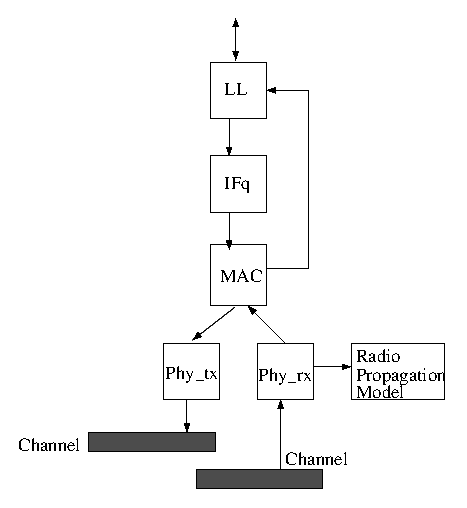
\includegraphics{sat-stack-basic}}
    \caption{Main components of a satellite network interface}
    \label{fig:sat-stack-basic}
\end{figure}

Satellite links resemble wireless links, which are described in Chapter
\ref{chap:mobility}.  Each satellite
node has one or more satellite network interface stacks, to which
channels are connected to the physical layer object in the stack.  Figure
\ref{fig:sat-stack-basic} illustrates the major components.  Satellite
links differ from \ns~wireless links in two major respects:  i) the
transmit and receive interfaces must be connected to different channels,
and ii) there is no ARP implementation.  Currently, the {\em
Radio Propagation Model} is a placeholder for users to add more detailed
error models if so desired; the current code does not use a propagation
model.

Network interfaces can be added with the following instproc of
\code{Class Node/SatNode}:
\begin{program}
$node add-interface $type $ll $qtype $qlim $mac $mac_bw $phy
\end{program}
The \code{add-interface} instproc returns an index value that can be used
to access the network interface stack later in the simulation.  By convention,
the first interface created on a node is attached to the uplink and downlink
channels of a satellite or terminal.  The
following parameters must be provided:

\begin{itemize} 
	\item {\bf type}:~~The following link types can be indicated:  
\code{geo} or 
\code{polar} for links from a terminal to a geo or polar satellite, 
respectively, \code{gsl} and \code{gsl-repeater} for links from a satellite
to a terminal, and \code{intraplane}, \code{interplane}, and \code{crossseam}
ISLs.  The type field is used internally in the simulator to identify the
different types of links, but structurally they are all very similar.
	\item {\bf ll}:~~The link layer type (\code{class LL/Sat} is currently
the only one defined).  
	\item {\bf qtype}:~~The queue type (e.g., \code{class Queue/DropTail}).
Any queue type may be used-- however, if additional parameters beyond the
length of the queue are needed, then this instproc may need to be modified
to include more arguments.
	\item {\bf qlim}:~~The length of the interface queue, in packets.
	\item {\bf mac}:~~The MAC type.  Currently, two types are defined:
\code{class Mac/Sat}-- a basic MAC for links with only one receiver (i.e.,
it does not do collision detection), and
\code{Class Mac/Sat/UnslottedAloha}-- an implementation of unslotted Aloha.
	\item {\bf mac\_bw}:~~The bandwidth of the link is set by this 
parameter, which controls the transmission time how fast the MAC sends. The
packet size used to calculate the transmission time is the sum of the
values \code{size()} in the common packet header and \code{LINK_HDRSIZE},
which is the size of any link layer headers.  The default value for
\code{LINK_HDRSIZE} is 16 bytes (settable in \code{satlink.h}).
The transmission time is encoded in the packet header for use at the
receive MAC (to simulate waiting for a whole packet to arrive).  
	\item {\bf phy}:~~The physical layer-- currently two Phys 
(\code{Class Phy/Sat} and \code{Class Phy/Repeater}) are defined.  
The class \code{Phy/Sat} just pass the information up and down the stack--
as in the wireless code described in Chapter \ref{chap:mobility}, 
a radio propagation model could be attached at this point.  The class
\code{Phy/Repeater} pipes any packets received on a receive interface
straight through to a transmit interface.
\end{itemize}

An ISL can be added between two nodes using the following instproc:
\begin{program}
$ns add-isl $ltype $node1 $node2 $bw $qtype $qlim
\end{program}
This creates two channels (of type \code{Channel/Sat}), and appropriate
network interfaces on both nodes, and attaches the channels to the 
network interfaces.  The bandwidth of the link is
set to \code{bw}.  The linktype (\code{ltype})
must be specified as either \code{intraplane}, \code{interplane}, or 
\code{crossseam}.


A GSL involves adding network interfaces and a channel on board the
satellite (this is typically done using the wrapper methods described
in the next paragraph), and then defining the correct interfaces on
the terrestrial node and attaching them to the satellite link, as 
follows:
\begin{program}
$node add-gsl $type $ll $qtype $qlim $mac $bw_up $phy \bs
   [$node_satellite set downlink_] [$node_satellite set uplink_]
\end{program}
Here, the \code{type} must be either \code{geo} or \code{polar}, 
and we make use
of the \code{downlink_} and \code{uplink_} instvars of the satellite;
therefore, the satellite's uplink and downlink must be created before
this instproc is called.

By default, the node generator for satellite nodes (described in
Section~\ref{sec:node:nodeconfig}) will create nodes of a 
given type, give them an uplink and
downlink interface, and create and attach an (initial) uplink and downlink
channel, based on the interface options specified.


%%%%%%%%%%%%%%%%%%%%%%%%%%%%%%%%%%%%%%%%%%%%%%%%%%%%%%%%%%%%%%%%%%%%%%%%%%

\subsection{Handoffs }
\label{sec:satellite/usage/handoffs}

Satellite handoff modelling is a key component of LEO satellite network 
simulations.  It is difficult to predict exactly how handoffs will occur
in future LEO systems because the subject is not well treated in the
literature.  In these satellite extensions, we establish certain criteria for 
handoffs, and allow nodes to independently monitor for situations that 
require a handoff.  An alternative would be to have all handoff events
synchronized across the entire simulation-- it would not be difficult to 
change the simulator to work in such a manner.

There are no link handoffs involving geostationary satellites, but there 
are two types of links to polar orbiting satellites
that must be handed off:  GSLs to polar satellites, and crossseam ISLs.  
A third type of link, interplane ISLs, are not handed off but are deactivated
at high latitudes as we describe below.

Each terminal connected to a polar orbiting satellite runs a timer that,
upon expiry, causes the \code{HandoffManager} to check whether the current 
satellite has fallen below the
elevation mask of the terminal.  If so, the handoff manager detaches the
terminal from that satellite's up and down links, and searches
through the linked list of satellite nodes for another possible satellite.
First, the ``next'' satellite in the current orbital plane is checked-- a 
pointer to this satellite is stored in the Position object of each
polar satellite node and is set during simulation configuration using
the \code{Node/SatNode} instproc ``\code{$node set_next $next_node}.''
If the next satellite is not suitable, the handoff manager searches
through the remaining satellites.  If it finds a suitable polar
satelite, it connects its network interfaces to that satellite's uplink and 
downlink channels, and restarts the handoff timer.  If it does not find 
a suitable
satellite, it restarts the timer and tries again later.  If any link
changes occur, the routing agent is notified.

The elevation mask and handoff timer interval are settable via OTcl: 
\begin{program}
HandoffManager/Term set elevation_mask_ 10; # degrees
HandoffManager/Term set term_handoff_int_ 10; # seconds
\end{program}
In addition, handoffs may be randomized to avoid phase effects by setting
the following variable:
\begin{program}
HandoffManager set handoff_randomization_ 0; # 0 is false, 1 is true 
\end{program}
If \code{handoff_randomization_} is true, then the next handoff interval
is a random variate picked from a uniform distribution across
$(0.5 * term\_handoff\_int\_, 1.5 * term\_handoff\_int\_)$.  

Crossseam ISLs are the only type of ISLs that are handed off.  The criteria
for handing off a crossseam ISL is whether or not there exists a satellite
in the neighboring plane that is closer to the given satellite than the
one to which it is currently connected.  Again, a handoff timer running
within the handoff manager on the polar satellite determines when the
constellation is checked for handoff opportunities.  Crossseam ISL
handoffs are
initiated by satellites in the lower-numbered plane of the two.  It is
therefore possible for a transient condition to arise in which a polar
satellite has two crossseam ISLs (to different satellites).  The
satellite handoff interval is again settable from OTcl and may also be
randomized:
\begin{program}
HandoffManager/Sat set sat_handoff_int_ 10; # seconds
\end{program}

Interplane and crossseam ISLs are deactivated near the poles, because 
the pointing requirements for the links are too severe as the satellite
draw close to one another.  Shutdown of these links is governed by a parameter:
\begin{program}
HandoffManager/Sat set latitude_threshold_ 70; # degrees 
\end{program}
The values for this parameter in the example scripts are speculative;
the exact value is dependent upon the satellite hardware.  The handoff
manager checks the latitude of itself and its peer satellite upon a handoff
timeout; if either or both of the satellites is above 
\code{latitude_threshold_} degrees latitude (north or south), the link
is deactivated until both satellites drop below this threshold.

Finally, if crossseam ISLs exist, there are certain situations in which
the satellites draw too close to one another in the mid-latitudes (if
the orbits are not close to being pure polar orbits).  We check for
the occurence of this orbital overlap with the following parameter:
\begin{program}
HandoffManager/Sat set longitude_threshold_ 10; # degrees 
\end{program}
Again, the values for this parameter in the example scripts are speculative.
If the two satellites are closer together in longitude than 
\code{longitude_threshold_} degrees, the link between them is deactivated.
This parameter is disabled (set to $0$) by default-- all defaults for
satellite-related bound variables can be found in \nsf{tcl/lib/ns-sat.tcl}.


%%%%%%%%%%%%%%%%%%%%%%%%%%%%%%%%%%%%%%%%%%%%%%%%%%%%%%%%%%%%%%%%%%%%%%%%%%

\subsection{Routing }
\label{sec:satellite/usage/routing}

The current status of routing is that it is incomplete.  Ideally, one should
be able to run all existing \ns~routing protocols over satellite links.  
However,
many of the existing routing protocols implemented in OTcl require that
the conventional \ns~links be used.  Contributions in this area are welcome,
but unfortunately it is not a trivial change.

With that being said, the current routing implementation is similar to
Session routing described in Chapter \ref{chap:unicast}, except that it
is implemented entirely in C++.   Upon each topology change, a centralized
routing genie determines the global network topology, computes new routes
for all nodes, and uses the routes to build
a forwarding table on each node.  Currently,
the slot table is kept by a routing agent on each node, and packets 
not destined for agents on the node are sent by default to this routing 
agent.  For each destination for which the node has a route, the forwarding
table contains a pointer to the head of the corresponding outgoing link.
As noted in Chapter \ref{chap:unicast}, the user is cautioned that this type 
of centralized routing can lead to minor causality violations.

The routing genie is a \code{class SatRouteObject} and is created and
invoked with the following OTcl commands:
\begin{program}
set satrouteobject_ [new SatRouteObject]
$satrouteobject_ compute_routes
\end{program}
where the call to \code{compute_routes} is performed after all of the
links and nodes in the simulator have been instantiated.
Like the \code{Scheduler}, there is one instance of a SatRouteObject in the
simulation, and it is accessed by means of an instance variable in C++.
For example, the call to recompute routes after a topology change is:
\begin{program}
SatRouteObject::instance().recompute();
\end{program}

Despite the current use of centralized routing, the design of having
a routing agent on each node was mainly done with distributed routing 
in mind.  Routing packets can be sent to port 255 of each node.  The key
to distributed routing working correctly is for the routing agent to
be able to 
determine from which link a packet arrived.  This is accomplished by the
inclusion of a \code{class NetworkInterface} object in each link, which
uniquely labels the link on which the packet arrived.  A helper function
\code{NsObject* intf_to_target(int label)} can be used to return the head 
of the
link corresponding to a given label.  The use of routing agents parallels
that of the mobility extensions, and the interested reader can turn to
those examples to see how to implement distributed routing protocols in
this framework.

The shortest-path route computations use the current propagation delay of
a link as the cost metric.  It is possible to compute routes using only
the hop count and not the propagation delays; in order to do so, set
the following default variable to "false":
\begin{program}
SatRouteObject set metric_delay_ "true"
\end{program}

Finally, for very large topologies (such as the Teledesic example), the 
centralized routing code will produce a very slow runtime because it executes
an all-pairs shortest path algorithm upon each topology change even if
there is no data currently being sent.  To speed up simulations in which
there is not much data transfer but there are lots of satellites and
ISLs, one can disable {\em handoff-driven} and enable {\em data-driven} 
route computations.  With data-driven computations, routes are computed
only when there is a packet to send, and furthermore, a single-source
shortest-path algorithm (only for the node with a packet to send) is 
executed instead of an all-pairs shortest path algorithm.  The following
OTcl variable can configure this option (which is set to "false" by
default):
\begin{program}
SatRouteObject set data_driven_computation_ "false"
\end{program}


%%%%%%%%%%%%%%%%%%%%%%%%%%%%%%%%%%%%%%%%%%%%%%%%%%%%%%%%%%%%%%%%%%%%%%%%%%

\subsection{Trace support}
\label{sec:satellite/usage/trace}

Tracefiles using satellite nodes and links are very similar to conventional
\ns~tracing described in Chapter \ref{chap:trace}.  Special SatTrace objects
(\code{class SatTrace} derives from \code{class Trace}) are used
to log the geographic latitude and longitude of the node logging the trace
(in the case of a satellite node, the latitude and longitude correspond
to the nadir point of the satellite).

For example, a packet on a link from node 66 to node 26 might normally be
logged as:  
\begin{program}
+ 1.0000 66 26 cbr 210 ------- 0 66.0 67.0 0 0 
\end{program}
but in the satellite simulation, the position information is appended:
\begin{program}
+ 1.0000 66 26 cbr 210 ------- 0 66.0 67.0 0 0 37.90 -122.30 48.90 -120.94
\end{program}
In this case, node 66 is at latitude 37.90 degrees, longitude -122.30
degrees, while node 26 is a LEO satellite whose subsatellite
point is at 48.90 degrees latitude, -120.94 degrees longitude (negative
latitude corresponds to south, while negative longitude corresponds to
west).

One addition is the \code{Class Trace/Sat/Error}, which traces any packets
that are errored by an error model.  The error trace logs packets dropped
due to errors as follows, for example:  
\begin{program}
e 1.2404 12 13 cbr 210 ------- 0 12.0 13.0 0 0 -0.00 10.20 -0.00 -10.00
\end{program}

It may happen that a satellite node generates a packet that it cannot
forward (such as in sat-mixed.tcl).  This will show up as a drop in
the tracefile with a destination field set to -2, and the coordinates
set to -999.00:
\begin{program}
d 848.0000 14 -2 cbr 210 ------- 1 14.0 15.0 6 21 0.00 10.00 -999.00 -999.00 
\end{program}
This indicates that node 14, in trying to send a packet to node 15, could
not find an available route.

To enable tracing of all satellite links in the simulator, use the following
commands {\em before} instantiating nodes and links:
\begin{program}
set f [open out.tr w]
$ns trace-all $f
\end{program}
Then use the following line after all node and link creation (and all
error model insertion, if any) to enable tracing of all satellite links:
\begin{program}
$ns trace-all-satlinks $f
\end{program}
Specifically, this will put tracing around the link layer queues in all
satellite links, and will put a receive trace between the mac and the
link layer for received packets.  To enable tracing only on a specific
link on a specific node, one may use the command:
\begin{program}
$node trace-inlink-queue $f $i
$node trace-outlink-queue $f $i
\end{program}
where $i$ is the index of the interface to be traced.  



The implementations of the satellite trace objects can be found in 
\nsf{tcl/lib/ns-sat.tcl} and \nsf{sattrace.\{cc,h\}}.

%%%%%%%%%%%%%%%%%%%%%%%%%%%%%%%%%%%%%%%%%%%%%%%%%%%%%%%%%%%%%%%%%%%%%%%%%%

\subsection{Error models}
\label{sec:satellite/usage/error}

\ns~error models are described in Chapter \ref{chap:error_model}.  These
error models can be set to cause packets to be errored according to various
probability distributions.  These error models are simple and don't 
necessarily correspond to what would be experienced on an actual satellite
channel (particularly a LEO channel).  Users are 
free to define more sophisticated error models that more closely match a 
particular satellite environment.

The following code provides an example of how to add an error model to a
link:
\begin{program}
set em_ [new ErrorModel]
$em_ unit pkt
$em_ set rate_ 0.02
$em_ ranvar [new RandomVariable/Uniform]
$node interface-errormodel $em_ 
\end{program}
This will add an error model to the receive path of the first interface
created on node \code{$node} (specifically, between the MAC and link layer)--
this first interface generally corresponds to the uplink and downlink
interface for a satellite or a terminal (if only one uplink and/or downlink
exists).
To add the error model to a different stack (indexed by $i$), use the 
following code:
\begin{program}
$node interface-errormodel $em_ $i 
\end{program}


%%%%%%%%%%%%%%%%%%%%%%%%%%%%%%%%%%%%%%%%%%%%%%%%%%%%%%%%%%%%%%%%%%%%%%%%%%

\subsection{Other configuration options}
\label{sec:satellite/usage/other}

Given an initial configuration of satellites specified for time $0$, 
it is possible to start the 
satellite configuration from any arbitrary point in time through the use of the
\code{time_advance_} parameter (this is really only useful for LEO
simulations). During the simulation run, this will set the position of 
the object to the position at time
\code{Scheduler::instance().clock + time_advance_} seconds.
\begin{program}
Position/Sat set time_advance_ 0; # seconds          
\end{program}


%%%%%%%%%%%%%%%%%%%%%%%%%%%%%%%%%%%%%%%%%%%%%%%%%%%%%%%%%%%%%%%%%%%%%%%%%%

\subsection{\nam~~support}
\label{sec:satellite/usage/nam}
\nam~~is not currently supported.  Addition of \nam~~ for satellite
is open to interested contributors.

%%%%%%%%%%%%%%%%%%%%%%%%%%%%%%%%%%%%%%%%%%%%%%%%%%%%%%%%%%%%%%%%%%%%%%%%%%

\subsection{Integration with wired and wireless code}
\label{sec:satellite/usage/integration}

Recently (November 2001), support has been added to connect traditional
OTcl-based wired nodes with the satellite nodes.  This section describes
the capabilities and limitations of that code.

The satellite code (and the wireless code) normally performs all routing 
in C++, while the traditional ns code uses a mix of OTcl and C++ code.   
For backward compatibility reasons, it is difficult to fully integrate
both the wired and wireless code.   The strategy for integrating wireless 
and wired code has been to define a special gateway node (called a 
"basestation"), to use hierarchial routing, and to locate a single basestation 
node in the wireless network with a network stack located in both the
wireless and the wired subnet.  Because routing is not fully integrated, 
the topology of the simulation is limited to only one gateway node per
wireless subnet (i.e., a packet cannot enter the wireless network from 
one wired gateway and leave via another).

The satellite/wired code integration takes a different strategy.  By
selecting the node configuration
\code{$ns node-config -wiredRouting ON} option, the C++
routing in the satellite code is turned off, and instead, all satellite 
topology changes lead to upcalls into the OTcl code.  As a result, 
the \code{link_} array in OTcl is manipulated according to all topology 
changes, and OTcl-based routing can occur.  The penalty for doing this 
is a much longer execution time for larger simulations (such as Teledesic), 
but for smaller simulations, the difference is not as noticeable.

An example script detailing the use of this new option is shown in
\nsf{tcl/ex/sat-wired.tcl}, and a similar test in the satellite test suite
exercises this code.  Additionally, all of the satellite example scripts
in \nsf{tcl/ex} directory can be converted to OTcl routing by using the 
\code{$ns node-config -wiredRouting ON} option.  However, there are a
few caveats: 
\begin{itemize}
\item The wired routing option for satellite has only been tested with
(the default) static routing: \code{$ns rtProto Static}.  The code triggers
a global routing table update upon any satellite topology change.
\item The option \code{data_driven_computation_}
can not be set to ``true'' when wiredRouting is ON.  Note that the enabling
or disabling of \code{data_driven_computation_}  can give subtle differences 
in simulation output since routes are computed at different times (while
propagation delays are continuously changing).  This effect can be seen
by toggling this parameter in the Iridium example 
script \nsf{tcl/ex/sat-iridium.tcl}.
\item In the trace file, when a packet is dropped due to ``no route to
host'' (such as when there is a topology change), the trace looks a bit
different depending on whether wiredRouting is turned OFF or ON.  In the
former case, there is one line per drop, with the destination labelled
as ``-2''.  In the latter case, there are three events (enque ``+'', 
deque ``-'', and drop ``d'') corresponding to the same packet, and the
destination is shown as ``-1''.  
\item In rare cases, there may be warning messages during the execution
indicating ``node out of range.''  This can occur if a node becomes
disconnected in the topology and then another node tries to send a packet
to it.  For example, try enabling \code{wiredRouting} in the file
\nsf{tcl/ex/sat-mixed.tcl}.  This occurs because the routing table is
dynamically sized upon topology change, and if a node becomes disconnected  
it may not have any entries inserted in the routing table (and hence
the routing table is not grown to accommodate its node number).  This
warning should not affect actual trace output.
\item There has been no attempt to interoperate with wireless or 
mobile-IP code.
\end{itemize}
 

%%%%%%%%%%%%%%%%%%%%%%%%%%%%%%%%%%%%%%%%%%%%%%%%%%%%%%%%%%%%%%%%%%%%%%%%%%

\subsection{Example scripts}
\label{sec:satellite/usage/example}

Example scripts can be found in the \nsf{tcl/ex} directory, including:
\begin{itemize}
\item \code{sat-mixed.tcl}  A simulation with a mixture of polar and
geostationary satellites.
\item \code{sat-wired.tcl}  Similar to the previous script, but shows how
to connect wired nodes to a satellite simulation.
\item \code{sat-repeater.tcl}  Demonstrates the use of a simple bent-pipe
geostationary satellite, and also error models.
\item \code{sat-aloha.tcl}  Simulates one hundred terminals in a mesh-VSAT
configuration using an unslotted Aloha MAC protocol 
with a ``bent-pipe'' geostationary satellite.  Terminals listen to their
own transmissions (after a delay), and if they do not successfully receive
their own packet within a timeout interval, they perform exponential 
backoff and then retransmit the packet. Three variants exist:
\code{basic}, \code{basic_tracing}, and \code{poisson}.  These variants
are described further in the header comments of the script.
\item \code{sat-iridium.tcl}  Simulates a broadband LEO constellation with
parameters similar to that of the Iridium constellation (with supporting
scripts \code{sat-iridium-links.tcl}, \code{sat-iridium-linkswithcross.tcl}, 
and \code{sat-iridium-nodes.tcl}).
\item \code{sat-teledesic.tcl}  Simulates a broadband LEO constellation with
parameters similar to those proposed for the 288 satellite Teledesic
constellation (with supporting scripts \code{sat-teledesic-links.tcl} and 
\code{sat-teledesic-nodes.tcl}).
\end{itemize}
In addition, there is a test suite script that tries to exercise a lot
of features simultaneously, it can be found at \nsf{tcl/test/test-suite-sat.tcl}.

%%%%%%%%%%%%%%%%%%%%%%%%%%%%%%%%%%%%%%%%%%%%%%%%%%%%%%%%%%%%%%%%%%%%%%%%%%
%%%%%%%%%%%%%%%%%%%%%%%%%%%%%%%%%%%%%%%%%%%%%%%%%%%%%%%%%%%%%%%%%%%%%%%%%%

\section{Implementation}
\label{sec:satellite/implementation}

The code for the implementation of satellite extensions can be found
in \nsf{\{sat.h, sathandoff.\{cc,h\}, satlink.\{cc,h\}, satnode.\{cc,h\}, 
satposition.\{cc,h\}, satroute.\{cc,h\}, sattrace.\{cc,h\}\}}, and
\nsf{tcl/lib/ns-sat.tcl}.  Almost all of the mechanism is implemented
in C++.

In this section, we focus on some of the key components of the implementation;
namely, the use of linked lists, the node structure, and a detailed look
at the satellite link structure.

\subsection{Use of linked lists}
\label{sec:satellite/implementation/list}

\begin{figure}
    \centerline{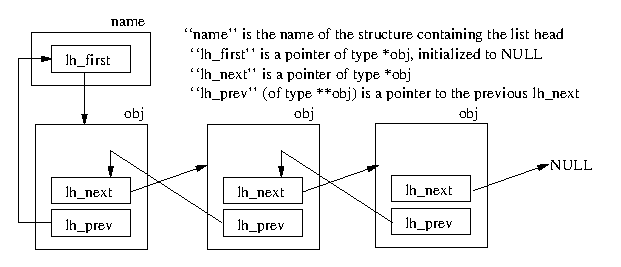
\includegraphics{linked-list}}
    \caption{Linked list implementation in \ns.}
    \label{fig:linked-list}
\end{figure}

There are a number of linked lists used heavily in the implementation:
\begin{itemize}

\item \code{class Node} maintains a (static) list of all objects of class
\code{Node} in the simulator.  The variable \code{Node::nodehead_} stores
the head of the list.  The linked list of nodes is used for centralized
routing, for finding satellites to hand off to, and for tracing.

\item \code{class Node} maintains a list of all (satellite) links on the
node.  Specifically, the list is a list of objects of class \code{LinkHead}. 
The variable \code{linklisthead_} stores the head of the list.  The
linked list of LinkHeads is used for checking whether or not to handoff
links, and to discover topology adjacencies.

\item \code{class Channel} maintains a list of all objects of class
\code{Phy} on the channel.  The head of the list is stored in the variable
\code{if_head_}.  This list is used to determine the set of interfaces on a
channel that should receive a copy of a packet.
\end{itemize}

Figure \ref{fig:linked-list} provides a schematic of how the linked list
is organized.  Each object in the list is linked through a ``LINK\_ENTRY''
that is a protected member of the class.  This entry contains a pointer
to the next item in the list and also a pointer to the address of the
previous ``next'' pointer in the preceding object.   Various macros
found in \nsf{list.h} can be used to manipulate the list; the 
implementation of linked-lists in \ns~is similar to the \code{queue} 
implementation found in some variants of BSD UNIX.

\subsection{Node structure}

\begin{figure}
    \centerline{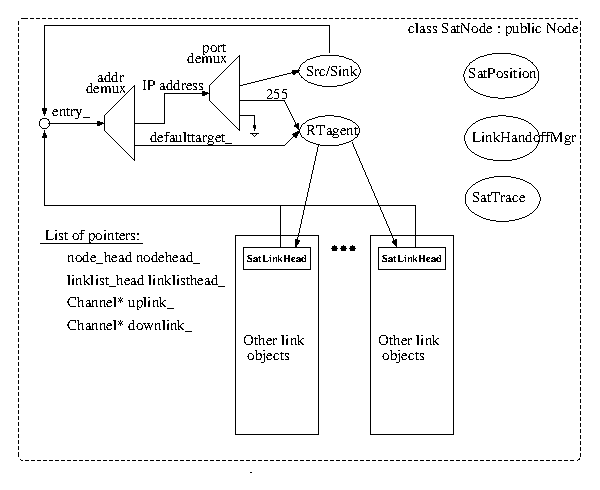
\includegraphics{sat-node}}
    \caption{Structure of \code{class SatNode}.}
    \label{fig:sat-node}
\end{figure}

Figure \ref{fig:sat-node} is a schematic of the main components of a
\code{SatNode}.  The structure bears resemblance to the \code{MobileNode}
in the wireless extensions, but there are several differences.  Like all
\ns~nodes, the SatNode has an ``entry'' point to a series of classifiers.
The address classifier contains a slot table for forwarding packets to 
foreign nodes, but since OTcl routing is not used, all packets not destined
for this node (and hence forwarded to the port classifier), are sent to
the default target, which points to a routing agent.  Packets destined
on the node for port 255 are classified as routing packets and are also
forwarded to the routing agent.

Each node contains one or more ``network stacks'' that include a generic
\code{SatLinkHead} at the entry point of the link.  The \code{SatLinkHead}
is intended to serve as an API to get at other objects in the link structure,
so it contains a number of pointers (although the API here has not been
finalized).  Packets leaving the network stack are sent to the node's
entry.  An important feature is that each packet leaving a network stack
has its \code{iface_} field in the common packet header coded with the
unique \code{NetworkInterface} index corresponding to the link.  This value
can be used to support distributed routing as described below.

The base class routing agent is \code{class SatRouteAgent}; it can be used 
in conjunction with centralized routing.  SatRouteAgents contain
a forwarding table that resolves a packet's address to a particular 
LinkHead target-- it is the job of the \code{SatRouteObject} to populate this
table correctly.  The SatRouteAgent populates certain fields in the header
and then sends the packet down to the approprate link.  To implement
a distributed routing protocol, a new SatRouteAgent could be defined-- this
would learn about topology by noting the interface index marked in each 
packet as it came up the stack-- a helper function in the node 
\code{intf_to_target()} allows it to resolve an index value to
a particular LinkHead. 

There are pointers to three additional objects in a SatNode.  First,
each SatNode contains a position object, discussed in the previous section.
Second, each SatNode contains a \code{LinkHandoffMgr} that monitors
for opportunities to hand links off and coordinates the handoffs.  Satellite
nodes and terminal nodes each have their specialized version of a 
LinkHandoffMgr.

Finally, a number of pointers to objects are contained in a SatNode.  We
discussed \code{linklisthead_} and \code{nodehead_} in the previous 
subsection.  The \code{uplink_} and \code{downlink_} pointers are
used for convenience under the assumption that, in most simulations,
a satellite or a terminal has only one uplink and downlink channel.

\subsection{Detailed look at satellite links}
\begin{figure}
    \centerline{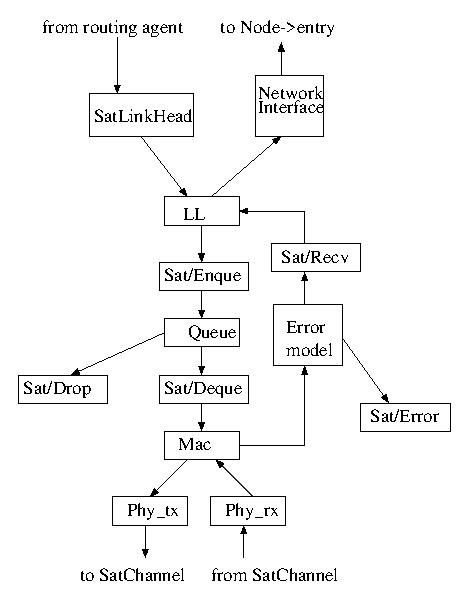
\includegraphics{sat-stack}}
    \caption{Detailed look at network interface stack.}
    \label{fig:sat-stack}
\end{figure}

Figure \ref{fig:sat-stack} provides a more detailed look at how satellite links
are composed.  In this section, we describe how packets move up and down
the stack, and the key things to note at each layer.  The file 
\nsf{tcl/lib/ns-sat.tcl} contains the various OTcl instprocs that assemble
links according to Figure \ref{fig:sat-stack}.  We describe the composite
structure herein as a ``network stack.''  Most of the code for the
various link components is in \nsf{satlink.\{cc,h\}}.

The entry point to a network stack is the \code{SatLinkHead} object.  The
SatLinkHead object derives from \code{Class LinkHead}; the aim of link
head objects is to provide a uniform API for all network stacks.
\footnote{In the author's opinion, all network stacks in \ns~ should 
eventually have a LinkHead object at the front-- the class SatLinkHead 
would then disappear.}  The SatLinkHead object contains pointers to
the LL, Queue, MAC, Error model, and both Phy objects.  The SatLinkHead
object can also be queried as to what type of network stack it is-- e.g.,
GSL, interplane ISL, crossseam ISL, etc..  Valid codes for the \code{type_} 
field are currently found in \nsf{sat.h}.  Finally, the SatLinkHead
stores a boolean variable \code{linkup_} that indicates whether
the link to at least one other node on the channel is up.  The C++
implementation of SatLinkHead is found in \nsf{satlink.\{cc,h\}}.

Packets leaving a node pass through the SatLinkHead transparently to the 
\code{class SatLL} object.  The SatLL class derives from LL (link layer).
Link layer protocols (like ARQ protocols) can be defined here.  The current
SatLL assigns a MAC address to the packet.  Note that in the satellite case,
we do not use an Address Resolution Protocol (ARP); instead, we simply use
the MAC \code{index_} variable as its address, and we use a helper function
to find the MAC address of the corresponding interface of the next-hop node.  
Since \code{class LL} derives from \code{class LinkDelay}, the \code{delay_}
parameter of LinkDelay can be used to model any processing delay in the
link layer; by default this delay is zero.

The next object an outgoing packet encounters is the interface queue.  
However, if tracing is enabled, tracing elements may surround the
queue, as shown in Figure \ref{fig:sat-stack}.  This part of a satellite
link functions like a conventional \ns~ link.

The next layer down is the MAC layer.  The MAC layer draws packets from
the queue (or deque trace) object-- a handshaking between the MAC and the 
queue allows the MAC to draw packets out of the queue as it needs them.  The
transmission time of a packet is modelled in the MAC also-- the MAC computes
the transmission delay of the packet (based on the sum of the 
LINK\_HDRSIZE field defined in \code{satlink.h} and the \code{size} field 
in the common packet header), and does not call up for another packet until
the current one has been ``sent'' to the next layer down.  Therefore, it
is important to set the bandwidth of the link correctly at this layer.
For convenience, the transmit time is encoded in the \code{mac} header; this
information can be used at the receiving MAC to calculate how long it must
wait to detect a collision on a packet, for example.

Next, the packet is sent to a transmitting interface (Phy\_tx) of class 
\code{SatPhy}.  This
object just sends the packet to the attached channel.  We noted earlier
in this chapter that all interfaces attached to a channel are part of the
linked list for that channel.  This is not true for transmit interfaces,
however.  Only receive interfaces attached to a channel comprise this linked
list, since only receive interfaces should get a copy of transmitted packets.
The use of separate transmit and receive interfaces mirrors the real world
where full-duplex satellite links are made up of RF channels at different
frequencies.

The outgoing packet is next sent to a \code{SatChannel}, which copies the
packet to every receiving interface (of class \code{SatPhy}) on the channel. 
The Phy\_rx sends the packet to the MAC layer.  At the MAC layer, the packet
is held for the duration of its transmission time (and any appropriate
collision detection is performed if the MAC, such as the Aloha MAC,
supports it).  If the packet is determined to have arrived safely at the MAC,
it next passes to an \code{ErrorModel} object, if it exists.  If not, the
packet moves through any receive tracing objects to the \code{SatLL}
object.  The SatLL object passes the packet up after a processing delay
(again, by default, the value for \code{delay_} is zero).

The final object that a received packet passes through is an object of
\code{class NetworkInterface}.  This object stamps the \code{iface_} field
in the common header with the network stack's unique index value.  This
is used to keep track of which network stack a packet arrived on.  The
packet then goes to the \code{entry} of the SatNode (usually, an address
classifier).  

Finally, ``geo-repeater'' satellites exist, as described earlier in this
chapter.  Geo-repeater network stacks are very simple-- they only contain
a Phy\_tx and a Phy\_rx of \code{class RepeaterPhy}, and a SatLinkHead.  
Packets received by a Phy\_rx are sent to the Phy\_tx without delay.  The
geo-repeater satellite is a degenerate satellite node, in that it does not
contain things like tracing elements, handoff managers, routing agents, or 
any other link interfaces other than repeater interfaces.


\section{Commands at a glance}
\label{sec:satcommands}

Following is a list of commands related to satellite networking:
\begin{flushleft}
\code{$ns_ node-config -satNodeType <type>}\\
This node configuration declares that the subsequent new nodes created
will be of type <type>, where <type> can be one of the following:
\code{geo, geo-repeater, polar, terminal}.  Other required fields for
satellite nodes (for setting up initial links and channels) are as follows 
(see Section~\ref{sec:node:nodeconfig}):
\code{$ns_ node-config -llType <type>}\\
\code{$ns_ node-config -ifqType <type>}\\
\code{$ns_ node-config -ifqLen <length>}\\
\code{$ns_ node-config -macType <type>}\\
\code{$ns_ node-config -channelType <type>}\\
\code{$ns_ node-config -downlinkBW <value>}\\

(note-- satNodeType geo-repeater only requires specifying the channelType-- all other options are disregarded.  See \code{tcl/ex/sat-repeater.tcl} for an example.)

\code{$ns_ satnode-polar <alt> <inc> <lon> <alpha> <plane> <linkargs> <chan>}\\
This a simulator wrapper method for creating a polar satellite node. Two
links, uplink and downlink, are created along with two channels, uplink
channel and downlink channel. <alt> is the polar satellite altitude,
<inc> is orbit inclination w.r.t equator, <lon> is the longitude of 
ascending node, <alpha>
gives the initial position of the satellite along this orbit, <plane> 
defines the plane of
the polar satellite. <linkargs> is a list of link argument options that
defines the network interface (like LL, Qtype, Qlim, PHY, MAC etc).


\code{$ns_ satnode-geo <lon> <linkargs> <chan>}\\
This is a wrapper method for creating a geo satellite node that first
creates a satnode plus two link interfaces (uplink and downlink) plus two 
satellite channels (uplink and downlink). <chan> defines the type of
channel.


\code{$ns_ satnode-geo-repeater <lon> <chan>}\\
This is a wrapper method for making a geo satellite repeater node that 
first creates a satnode plus two link interfaces (uplink and downlink)
plus two satellite channels (uplink and downlink). 


\code{$ns_ satnode-terminal <lat> <lon>}\\
This is a wrapper method that simply creates a terminal node. The <lat>
and <lon> defines the latitude and longitude respectively of the terminal.


\code{$ns_ satnode <type> <args>}\\
This is a more primitive method for creating satnodes of type <type>
which can be polar, geo or terminal. 


\code{$satnode add-interface <type> <ll> <qtype> <qlim> <mac_bw> <phy>}\\
This is an internal method of Node/SatNode that sets up link layer, mac
layer, interface queue and physical layer structures for the satellite
nodes.


\code{$satnode add-isl <ltype> <node1> <node2> <bw> <qtype> <qlim>}\\
This method creates an ISL (inter-satellite link) between the two nodes.
The link type (inter, intra or cross-seam), BW of the link, the queue-type
and queue-limit are all specified.


\code{$satnode add-gsl <ltype> <opt_ll> <opt_ifq> <opt_qlim> <opt_mac> <opt_bw> <opt_phy> <opt_inlink> <opt_outlink>}\\
This method creates a GSL (ground to satellite link). First a network
stack is created that is defined by LL, IfQ, Qlim, MAC, BW and PHY layers.
Next the node is attached to the channel inlink and outlink.


\end{flushleft}

\endinput


